% ------------------------------------------------------------------
\renewcommand{\thisunit}{MATH327 Unit 5}
\renewcommand{\moddate}{Last modified 4 Mar.~2025}
\setcounter{section}{5}
\setcounter{subsection}{0}
\phantomsection
\addcontentsline{toc}{section}{Unit 5: Thermodynamic cycles}
\section*{Unit 5: Thermodynamic cycles}
\subsection{\label{sec:work}Work, pressure and force}
In the previous section we defined the pressure of an ideal gas in the canonical ensemble as the thermodynamic response of the internal energy to an isentropic change in the volume (\eq{eq:pressure}).
We motivated this definition by thinking about `squeezing' the system --- exerting a force on it --- which suggests a connection between pressure and force.
Here we make this connection explicit by considering how the energy of an object changes when a force acts on it.

Let's begin by considering a single object at position $\vec r = (x, y, z)$, which is displaced by a vector $\d{\vec r}$ due to a force $\vec F(\vec r)$.
The \emph{work} done by this force is defined to be the resulting change in the energy of the object.
Infinitesimally, $W = \d{E} = \vec F\cdot \d{\vec r}$, which generalizes to the line integral $W = \De E = \int \vec F(r)\cdot d\vec r$.

A famous example is an object falling due to the force of the Earth's gravity.
That force is $\vec F = (0, 0, -mg)$, where $m$ is the mass of the object, $g \approx 9.8~\mathrm{m}/\mathrm{s}^2$ (metres per second per second) is the strength of gravity near the surface of the Earth, and the negative sign indicates that the gravitational force is directed downward.
Suppose the object starts from rest, with initial kinetic energy $E_0 = 0$, and falls downward, parallel to $\vec F$, from a height $h$.
Its final energy $E_f$ upon hitting the ground comes from the work done by the Earth's gravity:
\begin{align*}
  W & = \int \vec F(r)\cdot d\vec r = -mg \int_h^0 dz = mgh > 0 \\
  E_f & = E_0 + \De E = 0 + W = mgh = \frac{p_z^2}{2m} \qquad \lra \qquad p_z = -m\sqrt{2gh},
\end{align*}
where \eq{eq:momentum} relates the energy to the momentum $\vec p = (p_x, p_y, p_z)$.

\begin{shaded}
  Generalizing to $N \gg 1$ objects in a statistical system governed by the canonical ensemble, we define the \textbf{work} done by a force to be the resulting change in the system's average internal energy \textit{due to that force}, $W = \De\!\vev{E}_{\text{force}}$.
  In practice, the volume is the control parameter that such a force will change.
\end{shaded}

This change in $\vev{E}$ due to a change in volume suggests that the work is related to the pressure defined by \eq{eq:pressure}.
We can formalize this relation by considering the setup shown below (from Schroeder's \textit{Introduction to Thermal Physics}). \\[-24 pt]
\begin{center}
  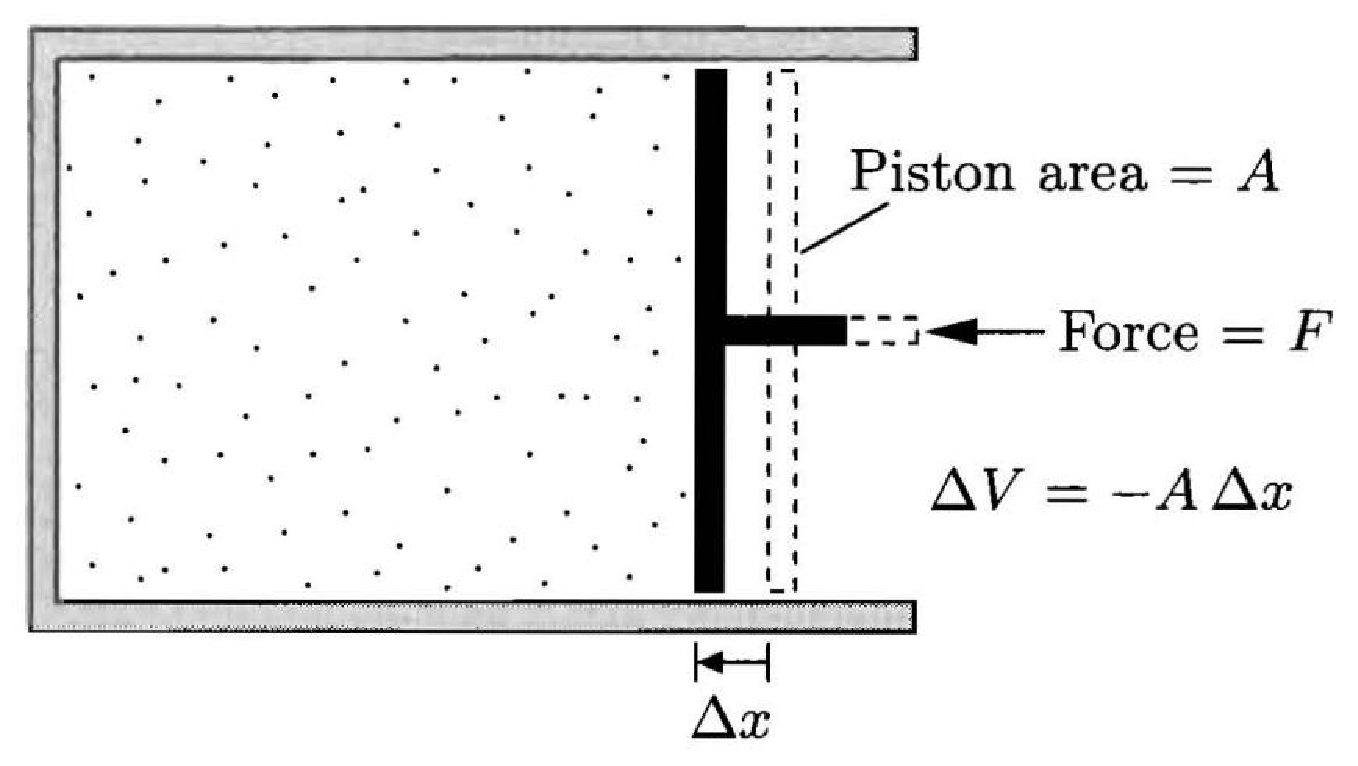
\includegraphics[width=0.54\textwidth]{figs/unit05_piston.pdf} % WARNING: ADJUSTED SIZE BY HAND TO FIT ON PAGE
\end{center}

Here we have an ideal gas in a container of volume $V$, with one wall of that container being a piston that we can move by applying a force $F$.
Let's demand that this process leaves the entropy of the gas constant.
The displacement $\De x > 0$ shown in the figure reduces the volume of the gas, by $\De V = -A\De x < 0$ where $A$ is the surface area of the piston.
Since the force $F$ is parallel to the piston's displacement $\De x$, it does positive work $W = F\De x > 0$.
Therefore the internal energy of the gas increases by $\De\!\vev{E} = W$, at the same time as its volume decreases isentropically, so from \eq{eq:pressure}
\begin{equation}
  P = -\left. \pderiv{}{V} \vev{E}\right|_S = -\frac{W}{\De V} = \frac{F\De x}{A\De x} = \frac{F}{A}.
\end{equation}
This identifies the pressure of an ideal gas in a container as the force per unit area that the gas exerts on the container wall, in agreement with our everyday experiences.

Rearranging the expressions above, we can obtain an expression for the work \textit{done on the gas by its surroundings} --- that is, by the external force applied to move the piston and change the volume.
Still assuming a constant-entropy (isentropic) process, this input work must match the increase in the gas's average internal energy,
\begin{align*}
  W & = \De\!\vev{E} = -P \De V & & \mbox{for constant entropy.}
\end{align*}
If the entropy is allowed to change, this relation between work and pressure will still hold.
However, as we will see in the next section, the non-constant entropy will introduce an additional change in the average internal energy unrelated to a force, leading to $W \neq \De\!\vev{E}$ and leaving only the relation
\begin{align}
  \label{eq:work_constP}
  W & = -P \De V & & \mbox{more generally.}
\end{align}
Later we will be interested in thermodynamic engines where work is \textit{done by the gas on its surroundings}.
This removes energy from the gas, corresponding to a negative $W < 0$, and we will need to be careful to keep track of the negative signs and their physical meaning.

Of course, as we change the volume of the gas, the pressure itself may change as described by the gas's equation of state --- such as the ideal gas law, \eq{eq:ideal_gas_law}.
In all these considerations we will keep the particle number $N$ fixed, though in principle it could change in the same way as discussed below \eq{eq:pressure} for the temperature.
With the equation of state providing an expression $P(V)$ for the pressure as a function of the volume, \eq{eq:work_constP} generalizes to
\begin{equation}
  \label{eq:work}
  W = -\int_{V_0}^{V_f} P(V) \d{V}.
\end{equation}
% ------------------------------------------------------------------



% ------------------------------------------------------------------
\subsection{Heat and entropy}
Now let's switch things up by changing the temperature $T$ of an ideal gas while keeping its volume $V$ and particle number $N$ constant.
Since the volume is constant, \eq{eq:work} indicates that no work is done, $W = 0$.
Even so, from \eq{eq:ideal_energy} we have $\vev{E} = \frac{3}{2} NT$ and can see that the average internal energy still changes,
\begin{equation}
  \label{eq:dE_dT}
  \d{\!\vev{E}} = \frac{3}{2} N \d{T}.
\end{equation}

In order to remain consistent with our discussion in the previous section, we should expect a change in the entropy to accompany this change in the internal energy that occurs with no work done.
Indeed, both distinguishable and indistinguishable particles lead to the same the temperature dependence in \eq{eq:ideal_entropy} for the entropy:
\begin{equation*}
  S = N\log\left(\lath^{-3}\right) + T\mbox{-independent} = N\log\left(T^{3 / 2}\right) + T\mbox{-independent}.
\end{equation*}
What is the change in entropy that results from changing the temperature by $dT$?
\begin{mdframed}
  $\displaystyle \d{S} = $ \\[50 pt]
\end{mdframed}
Looking back to \eq{eq:dE_dT}, you should find $\d{\!\vev{E}} = T \d{S}$, which leads us to another important definition.

\begin{shaded}
  The \textbf{heat} added to or removed from a statistical system is defined to be
  \begin{equation}
    \label{eq:heat_def}
    Q = T \d{S},
  \end{equation}
  and corresponds to the change in the average internal energy of the system when the volume and particle number are kept constant.
\end{shaded}

In the same way as our considerations of the work $W$ in the previous section, we can generalize this infinitesimal definition to
\begin{equation}
  \label{eq:heat}
  Q = \int_{S_0}^{S_f} T(S) \d{S},
\end{equation}
with $Q = \De\!\vev{E}$ when the volume is constant.
Here we assume it is possible to invert the usual canonical relation that expresses the entropy as a function of the temperature, $S(T)$.
Some textbooks may refer to infinitesimal heat and work as ``$\d{Q}$'' and ``$\d{W}$'', but this notation can easily be misinterpreted as describing a `change' in heat or work.
Instead, heat and work are themselves changes in the internal energy.

Like the work $W$, the heat $Q$ is positive when energy is added to the system to increase $\vev{E}$, and negative when energy is removed.
Recalling that the canonical ensemble involves placing the system in thermal contact with a large external thermal reservoir, we can recognize that this energy is not being created or destroyed, but is instead flowing back and forth between the system and the reservoir.
When considering heat, we will also demand that no \emph{entropy} is created or destroyed --- a positive $\d{S}$ will indicate entropy flowing into the system from the reservoir, while a negative value reflects entropy moving from the system to the reservoir.
Because the total entropy of the system plus its reservoir is constant, these processes are reversible, making it possible for the system to return to its starting macro-state.\footnote{In the case of irreversible processes, there must be sources of entropy creation, which change \eq{eq:heat_def} to $Q < T \d{S}$.  The \href{https://en.wikipedia.org/wiki/Clausius_theorem}{Clausius inequality} $Q \leq T \d{S}$ covers both reversible and irreversible cases.}

We have already considered isentropic processes with $\d{S} = 0$, for example in the definition of pressure in \eq{eq:pressure}.
With our assumption of reversibility, the definition of heat provides a new perspective on such processes:

\begin{shaded}
  We define an \textbf{adiabatic} process to be a change in the control parameters of a system that occurs without transferring heat, $Q = 0$.
  When this process is reversible, \eq{eq:heat_def} guarantees that it also does not change the system's entropy.
\end{shaded}

Since the canonical ensemble requires thermal contact between the system and its surroundings, the practical way to avoid heat exchange is to change the control parameters quickly.
That is, \textbf{adiabatic processes are fast} enough that the system does not have time to exchange heat (and hence entropy) with its surroundings.
The opposite extreme would be a process slow enough that any and all possible heat exchange can be completed while it is underway.
Based on our work in \secref{sec:heat_ex}, we can see that such heat exchange will keep the system's temperature equal to the temperature of its surroundings.
Taking that surrounding temperature to be constant, we reach the conclusion that \textbf{constant-temperature (or isothermal) processes are slow}.
Real processes generally exist in between these two extremes, usually closer to the adiabatic limit.
% ------------------------------------------------------------------



% ------------------------------------------------------------------
\subsection{Thermodynamic cycles}
Now we can generalize our considerations in the previous two sections to address simultaneous changes in the temperature $T$ and the volume $V$ of an ideal gas, still with fixed particle number $N$.
We are used to working with the internal energy $\vev{E}\!(T, V)$ and entropy $S(T, V)$ as functions of the temperature and volume.
Inverting the latter relation allows us to instead express the temperature $T(S, V)$ as a function of the entropy and volume, which carries through to the internal energy $\vev{E} = \frac{3}{2}NT$,
\begin{equation*}
  \vev{E}\!(T, V) \ \to \ \vev{E}\!(S, V).
\end{equation*}
Let's expand this to first order in a multi-variable Taylor expansion:
\begin{equation*}
  \vev{E}\!(S, V) \approx \vev{E}\!(S_0, V_0) + (S - S_0) \left.\pderiv{\vev{E}}{S}\right|_V + (V - V_0) \left.\pderiv{\vev{E}}{V}\right|_S.
\end{equation*}
This approximation becomes exact in the limit of infinitesimal changes
\begin{align*}
  \vev{E}\!(S, V) - \vev{E}\!(S_0, V_0) & \to \d{\!\vev{E}} \qquad &
  S - S_0 & \to \d{S} \qquad &
  V - V_0 & \to \d{V}. &
\end{align*}
At the same time, we can recognize the temperature from \eq{eq:temperature} and the (negative) pressure from \eq{eq:pressure}, to obtain
\begin{equation}
  \label{eq:first_law}
  d\!\vev{E} = T \d{S} - P \d{V} = Q + W.
\end{equation}
This is a generalized form of the \textbf{first law of thermodynamics}: Any change in the internal energy of a canonical system must be matched by (either or both) heat exchange with its surroundings or work done by or on those surroundings.

\begin{shaded}
  We now have all the concepts and \textbf{key equations} needed to consider a variety of ways to manipulate a canonical, classical, non-relativistic ideal gas in a container: \\[-24 pt]
  \begin{itemize}
    \item \eq{eq:ideal_energy} for the internal energy: \hfill $\vev{E} = \frac{3}{2} NT$
    \item \eq{eq:ideal_entropy} for the condition of constant entropy: \hfill $V T^{3/2} = \mbox{constant}$
    \item \eq{eq:ideal_gas_law} for the equation of state (ideal gas law): \hfill $PV = NT$
    \item \eq{eq:first_law} for the first law of thermodynamics: \hfill $d\!\vev{E} = T \d{S} - P \d{V} = Q + W$
  \end{itemize}
\end{shaded}

As examples of manipulations we can carry out by changing the system's control parameters, the piston we considered in \secref{sec:work} allows us to compress or expand the gas.
This change in volume could be fast to keep the entropy constant (adiabatic), or slow to keep the temperature constant (isothermal).
Alternatively, we can clamp the piston in place to keep the volume constant, and add heat to the gas to increase its temperature --- according to the ideal gas law, this will also increase the pressure of the gas.
Or we can add heat while keeping the pressure constant by applying a constant force to the piston.
The ideal gas law then implies the volume will increase, pushing out the piston and potentially doing work on the surroundings.

It's possible to carry out a sequence of such manipulations that cause the system to end up in the same thermodynamic (macro-)state in which it started, with the same pressure, volume, temperature and internal energy. % TODO: Could comment that this is related to our assumption of reversibility...
This sequence can then be repeated over and over again, always returning to the same starting point.
Such a repeatable process is known as a \textbf{thermodynamic cycle}.
As we will see in the next section, these cycles can make use of heat to have the system do work on its surroundings (providing an \textit{engine}), or make use of work to remove heat from the system (providing a \textit{refrigerator}), among other applications.

With $N$ fixed, the key equations above allow us to specify the full macro-state for an ideal gas solely in terms of the pressure $P$ and the volume $V$.
The ideal gas law provides the temperature $T = \frac{PV}{N}$, which then determines the internal energy $\vev{E} \propto NT$.
This makes it convenient to represent the system's macro-state as a point in a \textbf{pressure--volume} (or $\mathbf{PV}$) \textbf{diagram} --- a graph with the volume on the horizontal axis and the pressure on the vertical axis.
The manipulations discussed above correspond to lines in $PV$~diagrams.
In the case of a thermodynamic cycle, the lines must meet up to form a closed path for the system to go around as the cycle is repeated.

For example, the left figure on the next page shows the $PV$~diagram for isothermal expansion of the gas, which is slow enough for heat to enter the system to keep the temperature fixed despite the expansion.
\begin{center} % Don't need centering, but this will provide consistent vertical spacing
  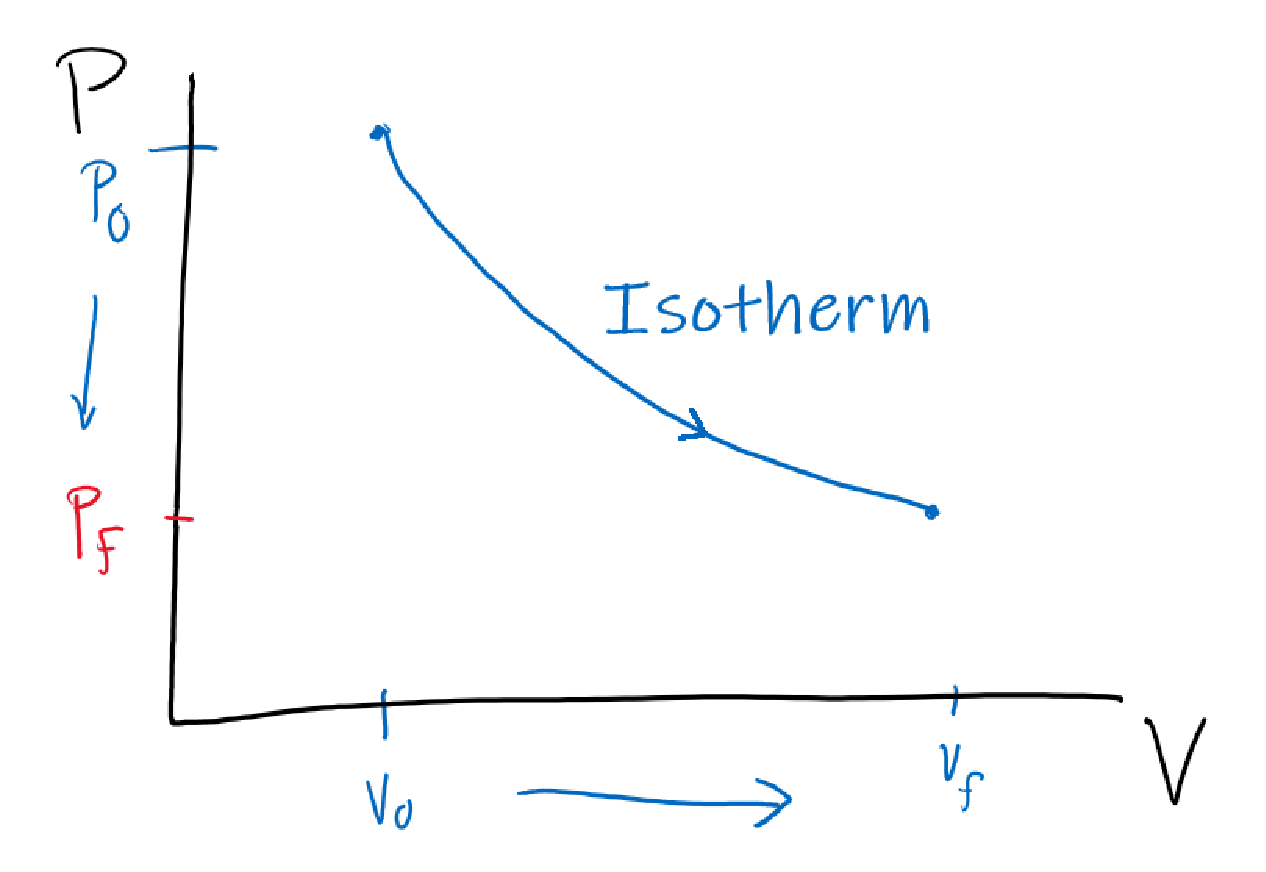
\includegraphics[width=0.475\textwidth]{figs/unit05_isotherm.pdf}\hfill 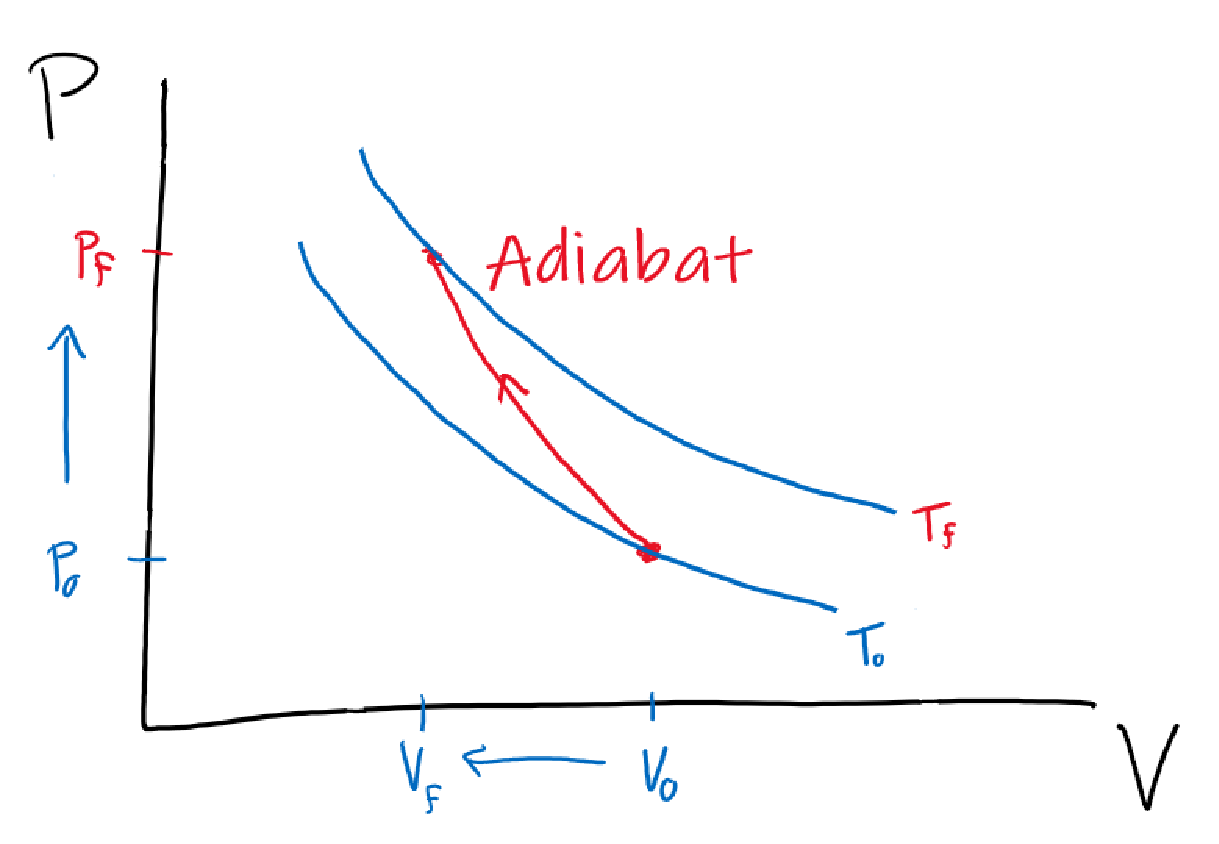
\includegraphics[width=0.475\textwidth]{figs/unit05_adiabat.pdf}
\end{center}
The line in a $PV$~diagram for an isothermal process is known as an \textit{isotherm}.
As the volume expands from $V_0$ to $V_f$, the temperature (and therefore $PV$) is constant.
What is the change in pressure $\De P = P_f - P_0$ in terms of $P_0$, $V_0$ and $V_f$?
What would it mean if two isotherms were to cross in a $PV$~diagram?
\begin{mdframed}
  \ \\[100 pt]
\end{mdframed}

Similarly, we can consider the $PV$~diagram on the right for adiabatic compression of the gas, which occurs too quickly for heat to be exchanged.
In this case both the pressure and temperature change, while the entropy (and therefore $VT^{3 / 2}$) is constant.
What are $\De P$ and the change in the temperature $\De T = T_f - T_0$ in terms of $P_0$, $V_0$, $V_f$ and the fixed number of particles $N$?
Can you convince yourself that two distinct reversible adiabats never cross? % physics.stackexchange.com/a/427582/34991 --- both adiabats intersect isotherms, but getting back to same entropy around cycle forbids heat flow to keep temperature constant on that isotherm
\begin{mdframed}
  \ \\[120 pt]
\end{mdframed}
% ------------------------------------------------------------------



% ------------------------------------------------------------------
\subsection{The Carnot cycle}
A famous thermodynamic cycle was proposed by \href{https://en.wikipedia.org/wiki/Nicolas_Leonard_Sadi_Carnot}{Sadi Carnot} in 1824, and laid the groundwork for subsequent development of engines and refrigerators later in the nineteenth century.
The key idea is to propose that the ideal gas in its container can exchange energy with either of \emph{two} different thermal reservoirs: a hot reservoir with a higher temperature $T_H$ and a cold reservoir with a lower temperature $T_L$. % Note 'C' reserved to refer to a point on the PV diagram below
The Carnot cycle consists of four stages, which are first shown below in the form of a $PV$~diagram, then illustrated in a sketch (adapted from Schroeder's \textit{Introduction to Thermal Physics}) that provides a more concrete picture of the physical processes, and finally summarized in words.

\begin{center}
  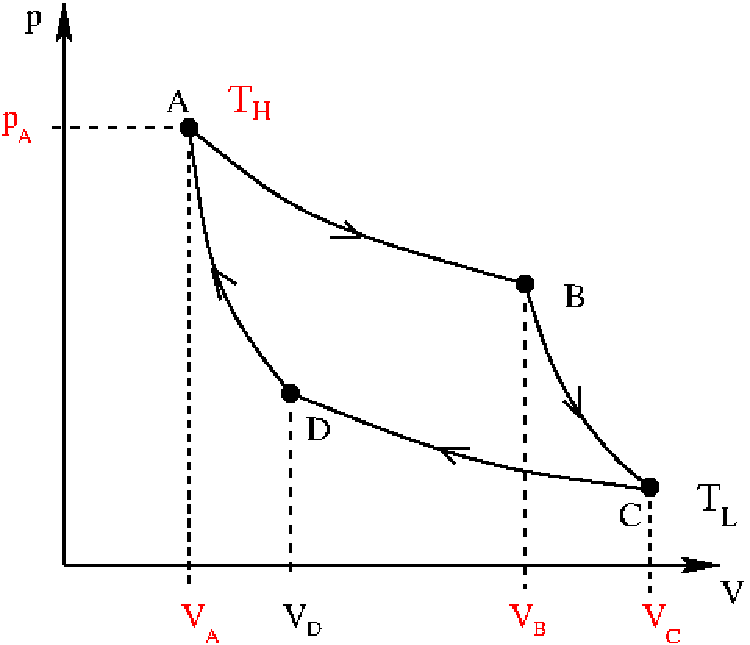
\includegraphics[width=0.75\textwidth]{figs/unit05_carnot-PV.pdf} \\[36 pt]
  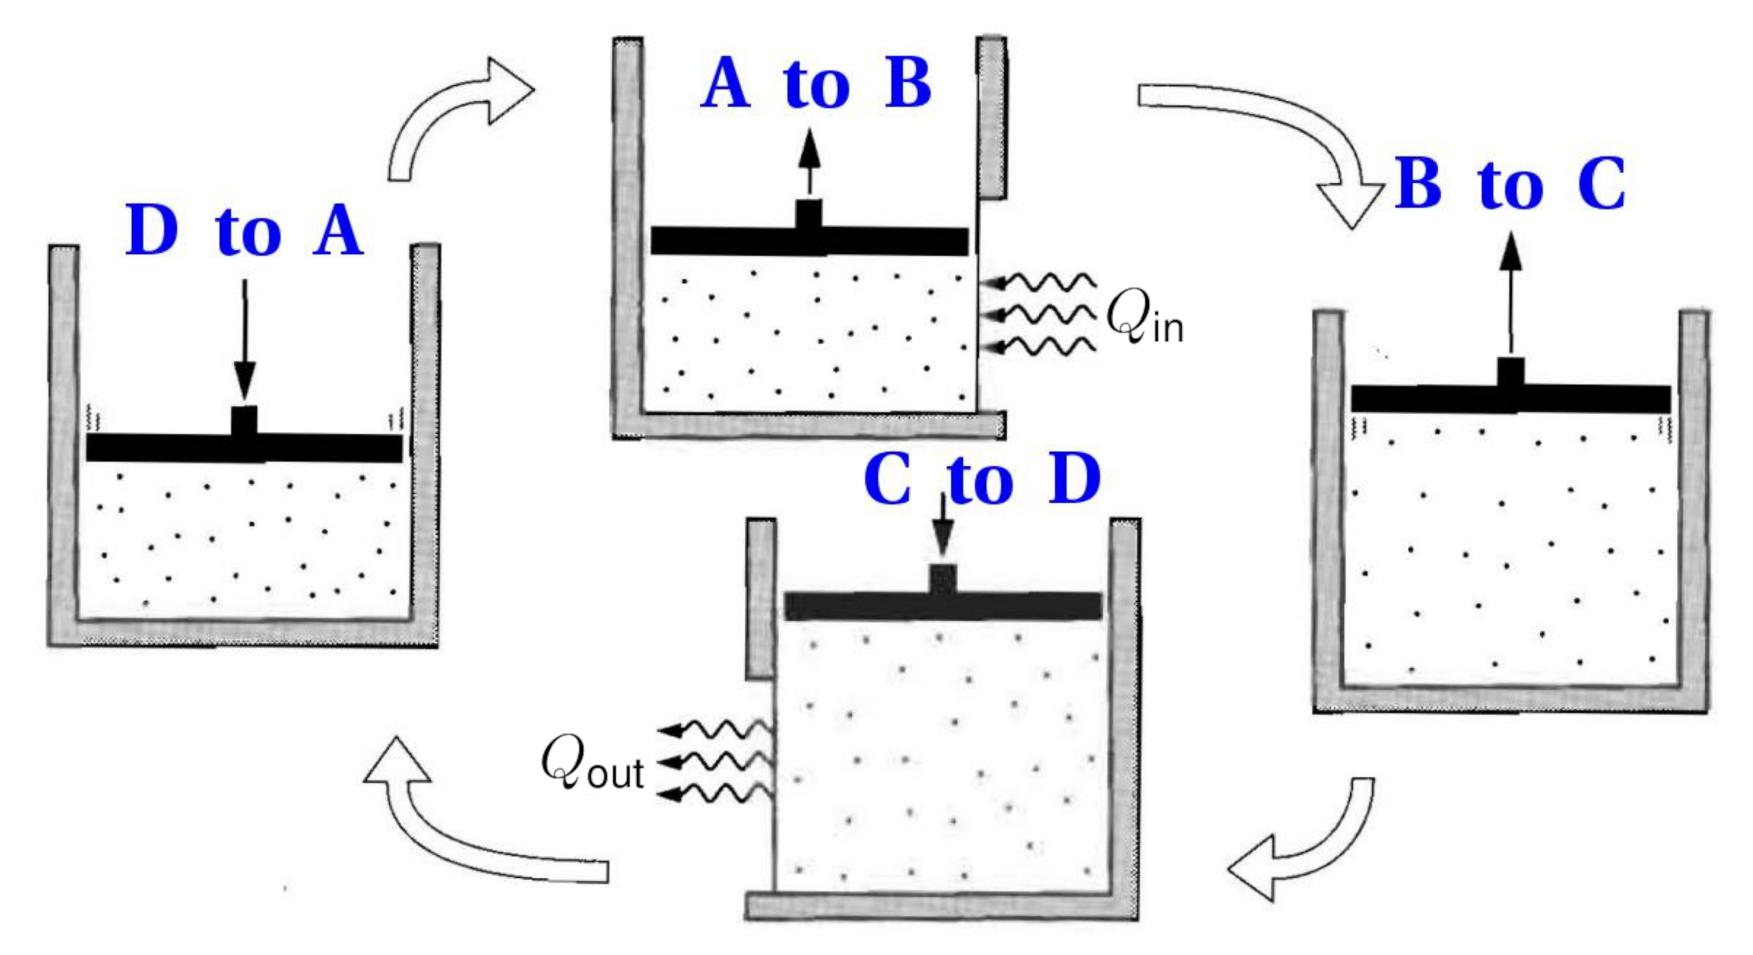
\includegraphics[width=\textwidth]{figs/unit05_carnot.pdf}
\end{center}

The illustration above supposes that the hot reservoir is located to the right of the system, while the cold reservoir is on its left.
In words, the four stages are the following: \\[-24 pt]
\begin{itemize}
  \item From point $A$ to point $B$ the system undergoes slow isothermal expansion, bringing in heat $Q_{\text{in}}$ from the hot reservoir in order to keep its temperature $T_H$ fixed.
  \item From point $B$ to point $C$ the system undergoes fast adiabatic expansion, with no heat exchange, until its temperature falls from $T_H$ down to $T_L$.
  \item From point $C$ to point $D$ the system undergoes slow isothermal compression, expelling heat $Q_{\text{out}}$ into the cold reservoir to keep its temperature $T_L$ fixed.
  \item From point $D$ to point $A$ the system undergoes fast adiabatic compression, with no heat exchange, until its temperature rises from $T_L$ back up to $T_H$.
\end{itemize}

We need to make sure that these processes really do produce a self-consistent closed cycle that our system could repeatedly follow.
In a real experiment, we would have full control over the four input variables $\left\{P_A, V_A, V_B, V_C\right\}$ coloured red in the $PV$~diagram above. % Could alternatively control temperatures...
Specifically, we can prepare our $N$-particle system in initial macro-state $A$ with our choice of pressure $P_A$ and volume $V_A$, which sets the higher temperature $T_H = \frac{P_A V_A}{N}$ of the hot reservoir.
We can then freely choose the volume $V_B > V_A$ at which to switch from isothermal expansion to adiabatic expansion, and similarly choose the volume $V_C > V_B$ at which we stop expanding and start compressing.
These choices of $V_B$ and $V_C$ set the lower temperature $T_L$ of the cold reservoir.

At this point, however, we are no longer free to choose an arbitrary volume $V_D < V_C$ at which to switch from isothermal compression to adiabatic compression --- this switch needs to happen at precisely the correct point in order for the final stage to bring the system back to its initial macro-state $A$.
While we can expect that this will be possible for the Carnot cycle, a priori there is no guarantee that a given sequence of processes will close to form a self-consistent thermodynamic cycle.

In order to confirm the self-consistency of the Carnot cycle, we need to express the unknown quantities $\left\{P_B, P_C, T_L, P_D, V_D\right\}$ in terms of the four inputs described above, along with the fixed number of particles $N$.
At point $B$, we know the system's temperature remains $T_H = P_A V_A / N$.
What is the pressure $P_B$ in terms of $\left\{P_A, V_A, V_B, V_C, N\right\}$?
\begin{mdframed}
  \ \\[100 pt]
\end{mdframed}

\newpage % WARNING: FORMATTING BY HAND
At point $C$, we know the system's entropy is the same as at point $B$.
What are the temperature $T_L$ and pressure $P_C$ in terms of $\left\{P_A, V_A, V_B, V_C, N\right\}$?
\begin{mdframed}
  \ \\[100 pt]
\end{mdframed}

At point $D$, we know the system's temperature remains $T_L$.
We have to demand that its entropy is the same as at point $A$, in order for the final adiabatic stage to connect points $D$ and $A$.
What are the resulting pressure $P_D$ and volume $V_D$ in terms of $\left\{P_A, V_A, V_B, V_C, N\right\}$?
\begin{mdframed}
  \ \\[100 pt]
\end{mdframed}

You should find that all of $\left\{P_B, P_C, T_L, P_D, V_D\right\}$ can be consistently specified by the inputs under our control, which confirms that the Carnot cycle is a valid thermodynamic cycle (as expected).
We now also have the ingredients needed to investigate how much net work (if any) this cycle can do on its surroundings, compared to the amount of heat it would transfer from the hot reservoir to the cold reservoir.
It will simplify this calculation to use the following positive quantities, with subscripts (rather than negative signs) indicating whether energy is flowing into or out of the gas: \\[-25 pt]
\begin{itemize}
  \setlength{\itemsep}{6pt}
  \setlength{\parskip}{0pt}
  \setlength{\parsep}{0pt}
  \item When work is done on the system by its surroundings, $W_{\text{in}} = W > 0$ from \eq{eq:work}
  \item When work is done by the system on its surroundings, $W_{\text{out}} = -W > 0$
  \item When heat enters the system, $Q_{\text{in}} = Q > 0$ from \eq{eq:heat}
  \item When heat leaves the system, $Q_{\text{out}} = -Q > 0$ \\[-25 pt]
\end{itemize}
We can now define a convenient combination of heat and work to consider.

\begin{shaded}
  The \textbf{efficiency} $\eta$ of a thermodynamic engine is defined to be
  \begin{equation}
    \label{eq:efficiency}
    \eta = \frac{W_{\text{done}}}{Q_{\text{in}}} = \frac{W_{\text{out}} - W_{\text{in}}}{Q_{\text{in}}},
  \end{equation}
  where $W_{\text{done}} = W_{\text{out}} - W_{\text{in}}$ is the \textit{net} amount of work done by each repetition of the cycle, while $Q_{\text{in}}$ is the \textit{total} amount of heat that enters the system in each repetition.
\end{shaded}

By specifying a thermodynamic \textit{engine}, we assume $W_{\text{out}} > W_{\text{in}}$, so that the overall cycle does more work on its surroundings than it requires to operate.
This corresponds to $\eta > 0$, and we can also put an upper bound on the efficiency, due to the first law of thermodynamics, \eq{eq:first_law}.
Because the system returns to its initial macro-state after each repetition of the cycle, we have
\begin{align}
  \De\!\vev{E} = 0 & = Q_{\text{in}} - Q_{\text{out}} + W_{\text{in}} - W_{\text{out}} \cr
                   & \Lra W_{\text{out}} - W_{\text{in}} = Q_{\text{in}} - Q_{\text{out}} \leq Q_{\text{in}}, \label{eq:cycle_heat_work}
\end{align}
or $\eta \leq 1$, with equality occurring when no `waste' heat is expelled during the cycle, so that $Q_{\text{out}} = 0$.
All together, $0 < \eta \leq 1$ lets us interpret the efficiency as the fraction of the incoming heat that the engine is able to use to do work on its surroundings.

We can illustrate these ideas by computing the efficiency of the Carnot cycle.
It is useful to divide this calculation into smaller pieces by considering the contributions to $W_{\text{done}}$ and $Q_{\text{in}}$ from each of the cycle's four stages.

First, in the isothermal expansion from point $A$ to point $B$, the ideal gas law provides $P(V)$ to insert into \eq{eq:work}:
\begin{mdframed}
  $\displaystyle W_{AB} = -\int_{V_A}^{V_B} P(V) \d{V} = $ \\[75 pt]
\end{mdframed}
You should find $W_{AB} < 0$, meaning the system does work on its surroundings during this stage.
At the same time, the constant temperature means $\De\!\vev{E} \propto \De T = 0$ from \eq{eq:ideal_energy}, so that $Q_{AB} = -W_{AB} > 0$, in agreement with our earlier observation of heat flowing into the system during this stage.

Next, in the adiabatic expansion from point $B$ to point $C$, we know $Q_{BC} = 0$, which lets us use the first law of thermodynamics to compute the work:
\begin{mdframed}
  $\displaystyle W_{BC} = $ \\[75 pt]
\end{mdframed}
You should find that the system continues doing work on its surroundings during this stage, $W_{BC} < 0$.

Finally, the computations for the two compression stages are directly analogous to those for the two expansion stages considered above.
For the isothermal compression from point $C$ to point $D$, the ideal gas law again provides $P(V)$:
\begin{mdframed}
  $\displaystyle W_{CD} = -\int_{V_C}^{V_D} P(V) \d{V} = $ \\[75 pt]
\end{mdframed}
Now you should find $W_{CD} > 0$, meaning this compression requires work to be done on the system by its surroundings, while $Q_{CD} = -W_{CD} < 0$ means heat flows out of the system.
For the adiabatic compression from point $D$ to point $A$, we know $Q_{DA} = 0$ while the change in temperature is exactly opposite the $\De T$ of the $B \to C$ adiabatic expansion.
Therefore $W_{DA} = -W_{BC} > 0$ and more work has to be done on the system to complete the cycle.

Putting everything together,
\begin{align}
  W_{\text{out}} & = -W_{AB} - W_{BC} \cr
  W_{\text{in}} & = W_{CD} + W_{DA} = W_{CD} - W_{BC} \cr
  Q_{\text{in}} & = Q_{AB} = -W_{AB} \cr
  \eta & = \frac{-W_{AB} - W_{BC} - W_{CD} + W_{BC}}{-W_{AB}} = 1 + \frac{W_{CD}}{W_{AB}} = 1 - \frac{T_L}{T_H}.
\end{align}
We can check that our result $\eta = 1 - \frac{T_L}{T_H}$ for the efficiency of the Carnot cycle makes sense.
Since $T_L < T_H$, we have $\eta > 0$.
If the temperatures of the hot and cold reservoirs approach each other, $\frac{T_L}{T_H} \to 1$, then the cycle would collapse to a single isotherm with $W_{\text{out}} = W_{\text{in}}$ and vanishing efficiency $\eta \to 0$.
In the opposite limit of a large difference in the temperatures $T_L \ll T_H$, the efficiency would improve, with $\eta \to 1$ as $\frac{T_L}{T_H} \to 0$.

It turns out to be generic for heat engines to operate more efficiently as the temperature difference between their hot and cold reservoirs increases, and they always cease performing net work as $\frac{T_L}{T_H} \to 1$.
The Carnot cycle is special because its efficiency $\eta = 1 - \frac{T_L}{T_H}$ is the theoretical maximum allowed by the second law of thermodynamics.
We can show this by using \eq{eq:cycle_heat_work} to rewrite
\begin{equation*}
  \eta = \frac{Q_{\text{in}} - Q_{\text{out}}}{Q_{\text{in}}} = 1 - \frac{Q_{\text{out}}}{Q_{\text{in}}} = 1 - \frac{T_L \De S_{\text{out}}}{T_H \De S_{\text{in}}},
\end{equation*}
where the last equality uses \eq{eq:heat} and the fact that the input heat $Q_{\text{in}} = T_H \De S_{\text{in}}$ enters the engine from the hot reservoir with temperature $T_H$, while the waste heat $Q_{\text{out}} = T_L \De S_{\text{out}}$ is expelled to the cold reservoir with temperature $T_L$.
After each repetition of the cycle, the gas returns to its original macro-state, with its original entropy, after absorbing entropy $\De S_{\text{in}}$ from its surroundings and expelling $\De S_{\text{out}}$ back out again.
The second law therefore demands $\De S_{\text{out}} \geq \De S_{\text{in}}$, so that
\begin{equation*}
  \eta = 1 - \frac{T_L}{T_H} \frac{\De S_{\text{out}}}{\De S_{\text{in}}} \leq 1 - \frac{T_L}{T_H}
\end{equation*}
in principle, for any thermodynamic engine. % TODO: Equality implied for any completely reversible process --- otherwise would need additional entropy to close cycle, for instance by burning fuel

Finally, if we were to operate the Carnot cycle in reverse, with isothermal expansion at temperature $T_L$ and compression at $T_H$, we would do work on the system in order to bring heat in from the cold reservoir (i.e., $Q_{\text{in}} = T_L \De S_{\text{in}}$) and expel it into the hot reservoir ($Q_{\text{out}} = T_H \De S_{\text{out}}$).
In other words, we would have a refrigerator rather than an engine.
The `efficiency' of a refrigerator is called its \textit{coefficient of performance}, and defined as
\begin{equation*}
  \mathrm{COP} = \frac{Q_{\text{in}}}{W_{\text{in}} - W_{\text{out}}} = \frac{Q_{\text{in}}}{Q_{\text{out}} - Q_{\text{in}}} = \frac{1}{Q_{\text{out}} / Q_{\text{in}} - 1} \leq \frac{1}{T_H / T_L - 1} = \frac{T_L}{T_H - T_L},
\end{equation*}
which can be greater than one.
The reversed Carnot cycle provides the best possible $\mathrm{COP}$ for a refrigerator.
Despite its efficiency, the Carnot cycle does not provide a practical engine or refrigerator, simply because its slow isothermal stages take too long!
Real engines and refrigerators sacrifice efficiency for functionality.
% ------------------------------------------------------------------
